%%%%%%%%%%%%%%%%%%%%%%%%%%%%%%%%%%%%%%%%%%%%%%%%%%%%%%%%%%%%%%%%%%%%%%%%%%%%%%%%%%%%%%%%%
% Autor:        Aguilar Enriquez, Paul Sebastian a.k.a. Penserbjorne
% Autor:        @yesn7
% Fecha:        05/02/2017
% Descripcion:  Plantilla base para actividades o tareas.
%%%%%%%%%%%%%%%%%%%%%%%%%%%%%%%%%%%%%%%%%%%%%%%%%%%%%%%%%%%%%%%%%%%%%%%%%%%%%%%%%%%%%%%%%

\documentclass[a4paper,11pt]{article}                 % Papel tamaño carta, texto de 11pt.

\usepackage[top=2cm, bottom=2cm, left=2.2cm, right=2.2cm]{geometry} % Margenes
\usepackage[T1]{fontenc}                              % Indicamos la codificacion de las fuentes.
\usepackage[utf8x]{inputenc}                          % Definimos la codificacion.
\usepackage{lmodern}                                  % Para poder usar acentos.
\usepackage[spanish]{babel}                           % Usaremos idioma español.
\usepackage{amsmath}                                  % Para formulas matematicas.
\usepackage{graphicx}                                 % Para imagenes.
\usepackage{float}                                    % Para posicionar objetos.
\usepackage{booktabs}                                 % Para formatear tablas.
\usepackage{hyperref}                                 % Para enlaces y referencias.
\usepackage{lscape}
\usepackage[table,xcdraw]{xcolor}
 %\usepackage{timetable}
% \usepackage[spanish.mexico]{babel}
\usepackage{tabularx}
\usepackage{multirow}
% \usepackage[table,xcdraw]{xcolor}
\usepackage{longtable}
\usepackage{lipsum}


%%%%%%%%%%%%%%%%%%%%%%%%%%%%%%%%%%%%%%%%%%%%%%%%%%%%%%%%%%%%%%%%%%%%%%%%%%%%%%%%%%%%%%%%%

% Los logos tienen posiciones relativas al nombre de la escuela.
% Cada imagen esta desplazada con respecto al texto, en este caso nombre de la univseridad.
% No se necesitan paquetes adicionales, el entorno estandar para imagenes de LaTeX puede hacerlo.
% El truco esta en definir una imagen de tamaño cero, asi no afecta al centrar los titulos.
\def\logoUNAM{%
  \begin{picture}(0,0)\unitlength=1cm
    \put (-3.5,-3) {
\includegraphics[width=8em]{images/escudo-unam}}
  \end{picture}
}

\def\logoFI{%
  \begin{picture}(0,0)\unitlength=1cm
    \put (0.5,-3) {
\includegraphics[width=8em]{images/escudo-fi}}
  \end{picture}
}

%%%%%%%%%%%%%%%%%%%%%%%%%%%%%%%%%%%%%%%%%%%%%%%%%%%%%%%%%%%%%%%%%%%%%%%%%%%%%%%%%%%%%%%%%

\author{LIDSOL}  % Autor de la actividad.
\title{Reporte 2018}                % Titulo de la actividad.

\date{13/06/2018}                                           % Fecha de entrega.

                                          % Fecha de entrega.

\def\universidad{Universidad Nacional Autónoma de México}   % Nombre de la universidad.
\def\facultad{Facultad de Ingeniería}                              % Nombre de la facultdad.
\def\semestre{2018}                                     % Semestre lectivo.
\def\materia{Laboratorio de Investigación y Desarrollo del Software Libre}               % Nombre de la materia y grupo.
\makeatletter

%%%%%%%%%%%%%%%%%%%%%%%%%%%%%%%%%%%%%%%%%%%%%%%%%%%%%%%%%%%%%%%%%%%%%%%%%%%%%%%%%%%%%%%%%

\begin{document}
  
  % Titulo del documento con logos.
  \begin{center}
    \logoUNAM {\Large \universidad} \logoFI\par
    {\large \facultad}\par

    \materia\par
    \semestre\par
   % \@author\par
    \@date\par
    \@title
  \end{center}

  \hrulefill\par

  \pagenumbering{gobble}                              % Oculta el numero de pagina.
  \tableofcontents                                    % Crea el indice o tabla de contenido.

%%%%%%%%%%%%%%%%%%%%%%%%%%%%%%%%%%%%%%%%%%%%%%%%%%%%%%%%%%%%%%%%%%%%%%%%%%%%%%%%%%%%%%%%%

  \newpage
  \pagenumbering{arabic} 
                                 % Muestra el numero de pagina.
  \section{Inventario}
  \subsection{Inventario a Octubre del 2016}
  \subsubsection*{Papelería}
    \begin{table}[H]
    \centering
    % \caption{My caption}
    % \label{my-label}
    \begin{tabular}{|c|l|}
    \hline
    Cantidad & \multicolumn{1}{c|}{Descripción} \\ \hline
    4        & Cintas masking tape 1”           \\ \hline
    1        & Cinta masking tape 1/2”          \\ \hline
    1        & Cinta scotch transparente 1”     \\ \hline
    1        & Pintarrón                        \\ \hline
    7        & Plumones para pintarrón          \\ \hline
    2        & Borradores para pintarrón        \\ \hline
    \end{tabular}
    \end{table}
  \subsubsection*{Anaquel blanco}
    \begin{table}[H]
    \centering
    % \caption{My caption}
    % \label{my-label}
    \begin{tabular}{|c|l|}
    \hline
    Cantidad & Descripción                                                                     \\ \hline
    1        & Anaquel blanco                                                                  \\ \hline
    1        & Botiquín de primeros auxilios                                                   \\ \hline
    1        & Impresora HP Laserjet (sin cable de alimentación)                               \\ \hline
    1        & Paquete sellado con cinta canel con cargador y varios cables                    \\ \hline
    1        & Mouse HP                                                                        \\ \hline
    1        & Varios papeles (Catálogo de lenguas indígenas, engargolados, carpetas, gacetas) \\ \hline
    1        & Tarjeta de red en bolsa antiestatica                                            \\ \hline
    1        & Balon de futbol                                                                 \\ \hline  
    1        & Bote con producto de limpieza                                                   \\ \hline  
    1        & Montón de varios discos                                                         \\ \hline
    \end{tabular}
    \end{table} 
    \begin{figure}[H]
      \centering                            
      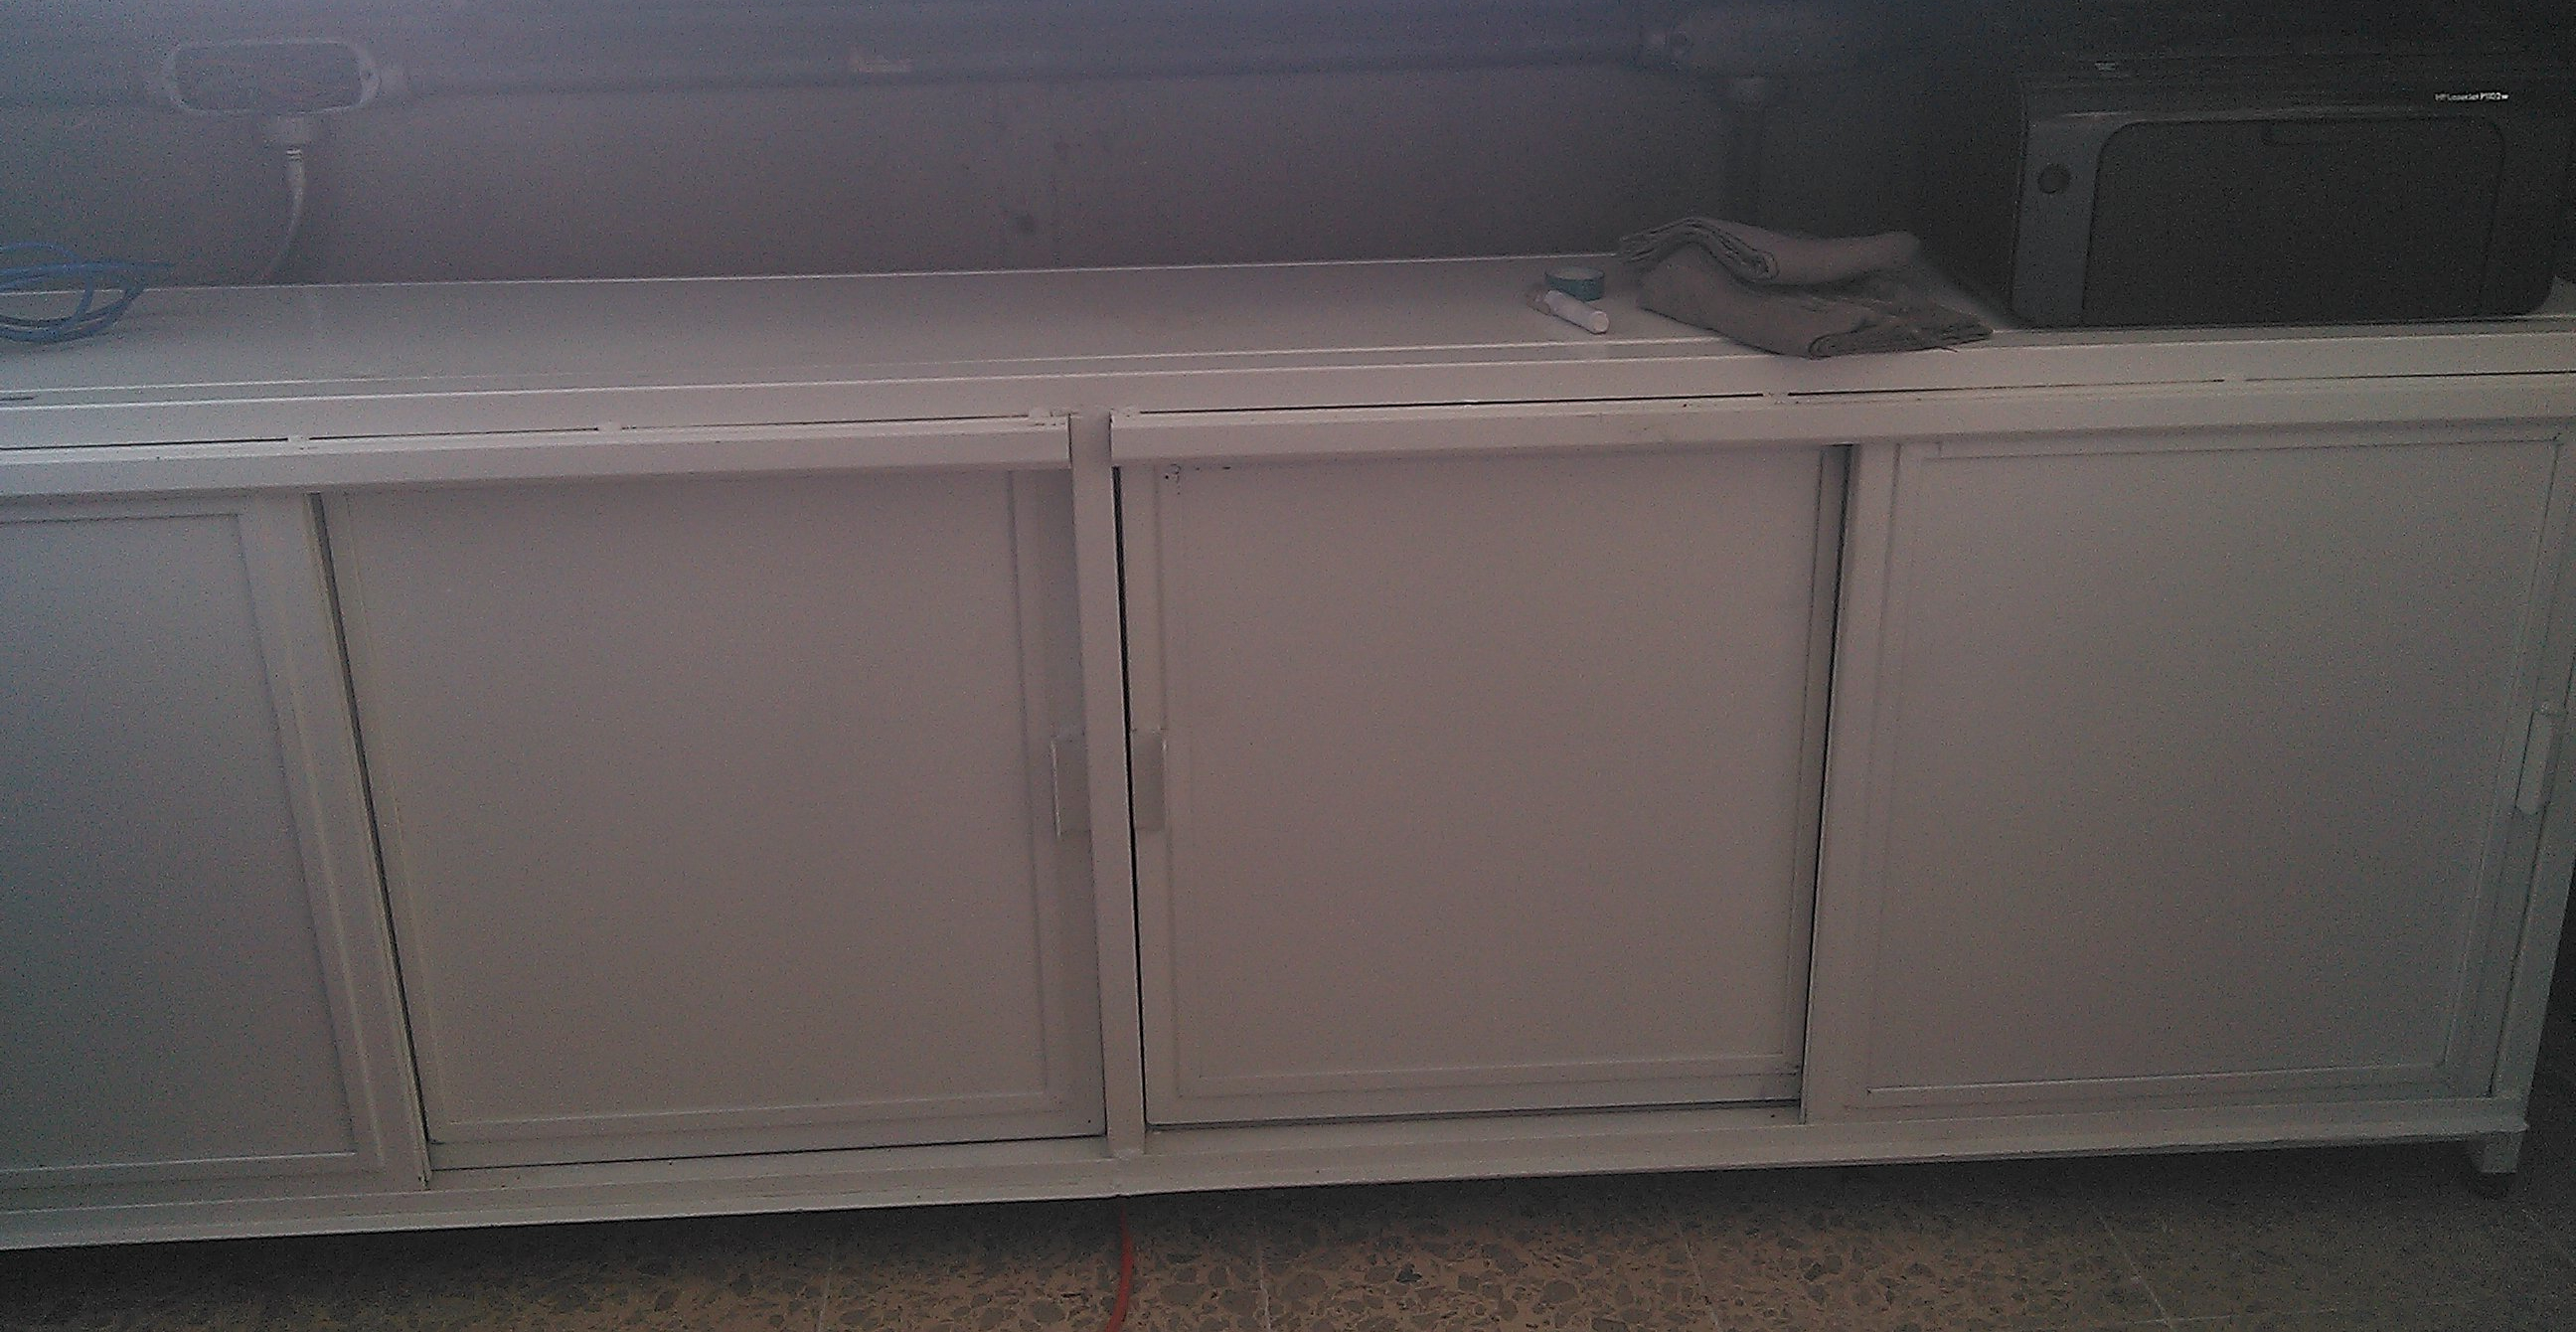
\includegraphics[width=0.6\textwidth]{images/anaquel-blanco-01} \\
      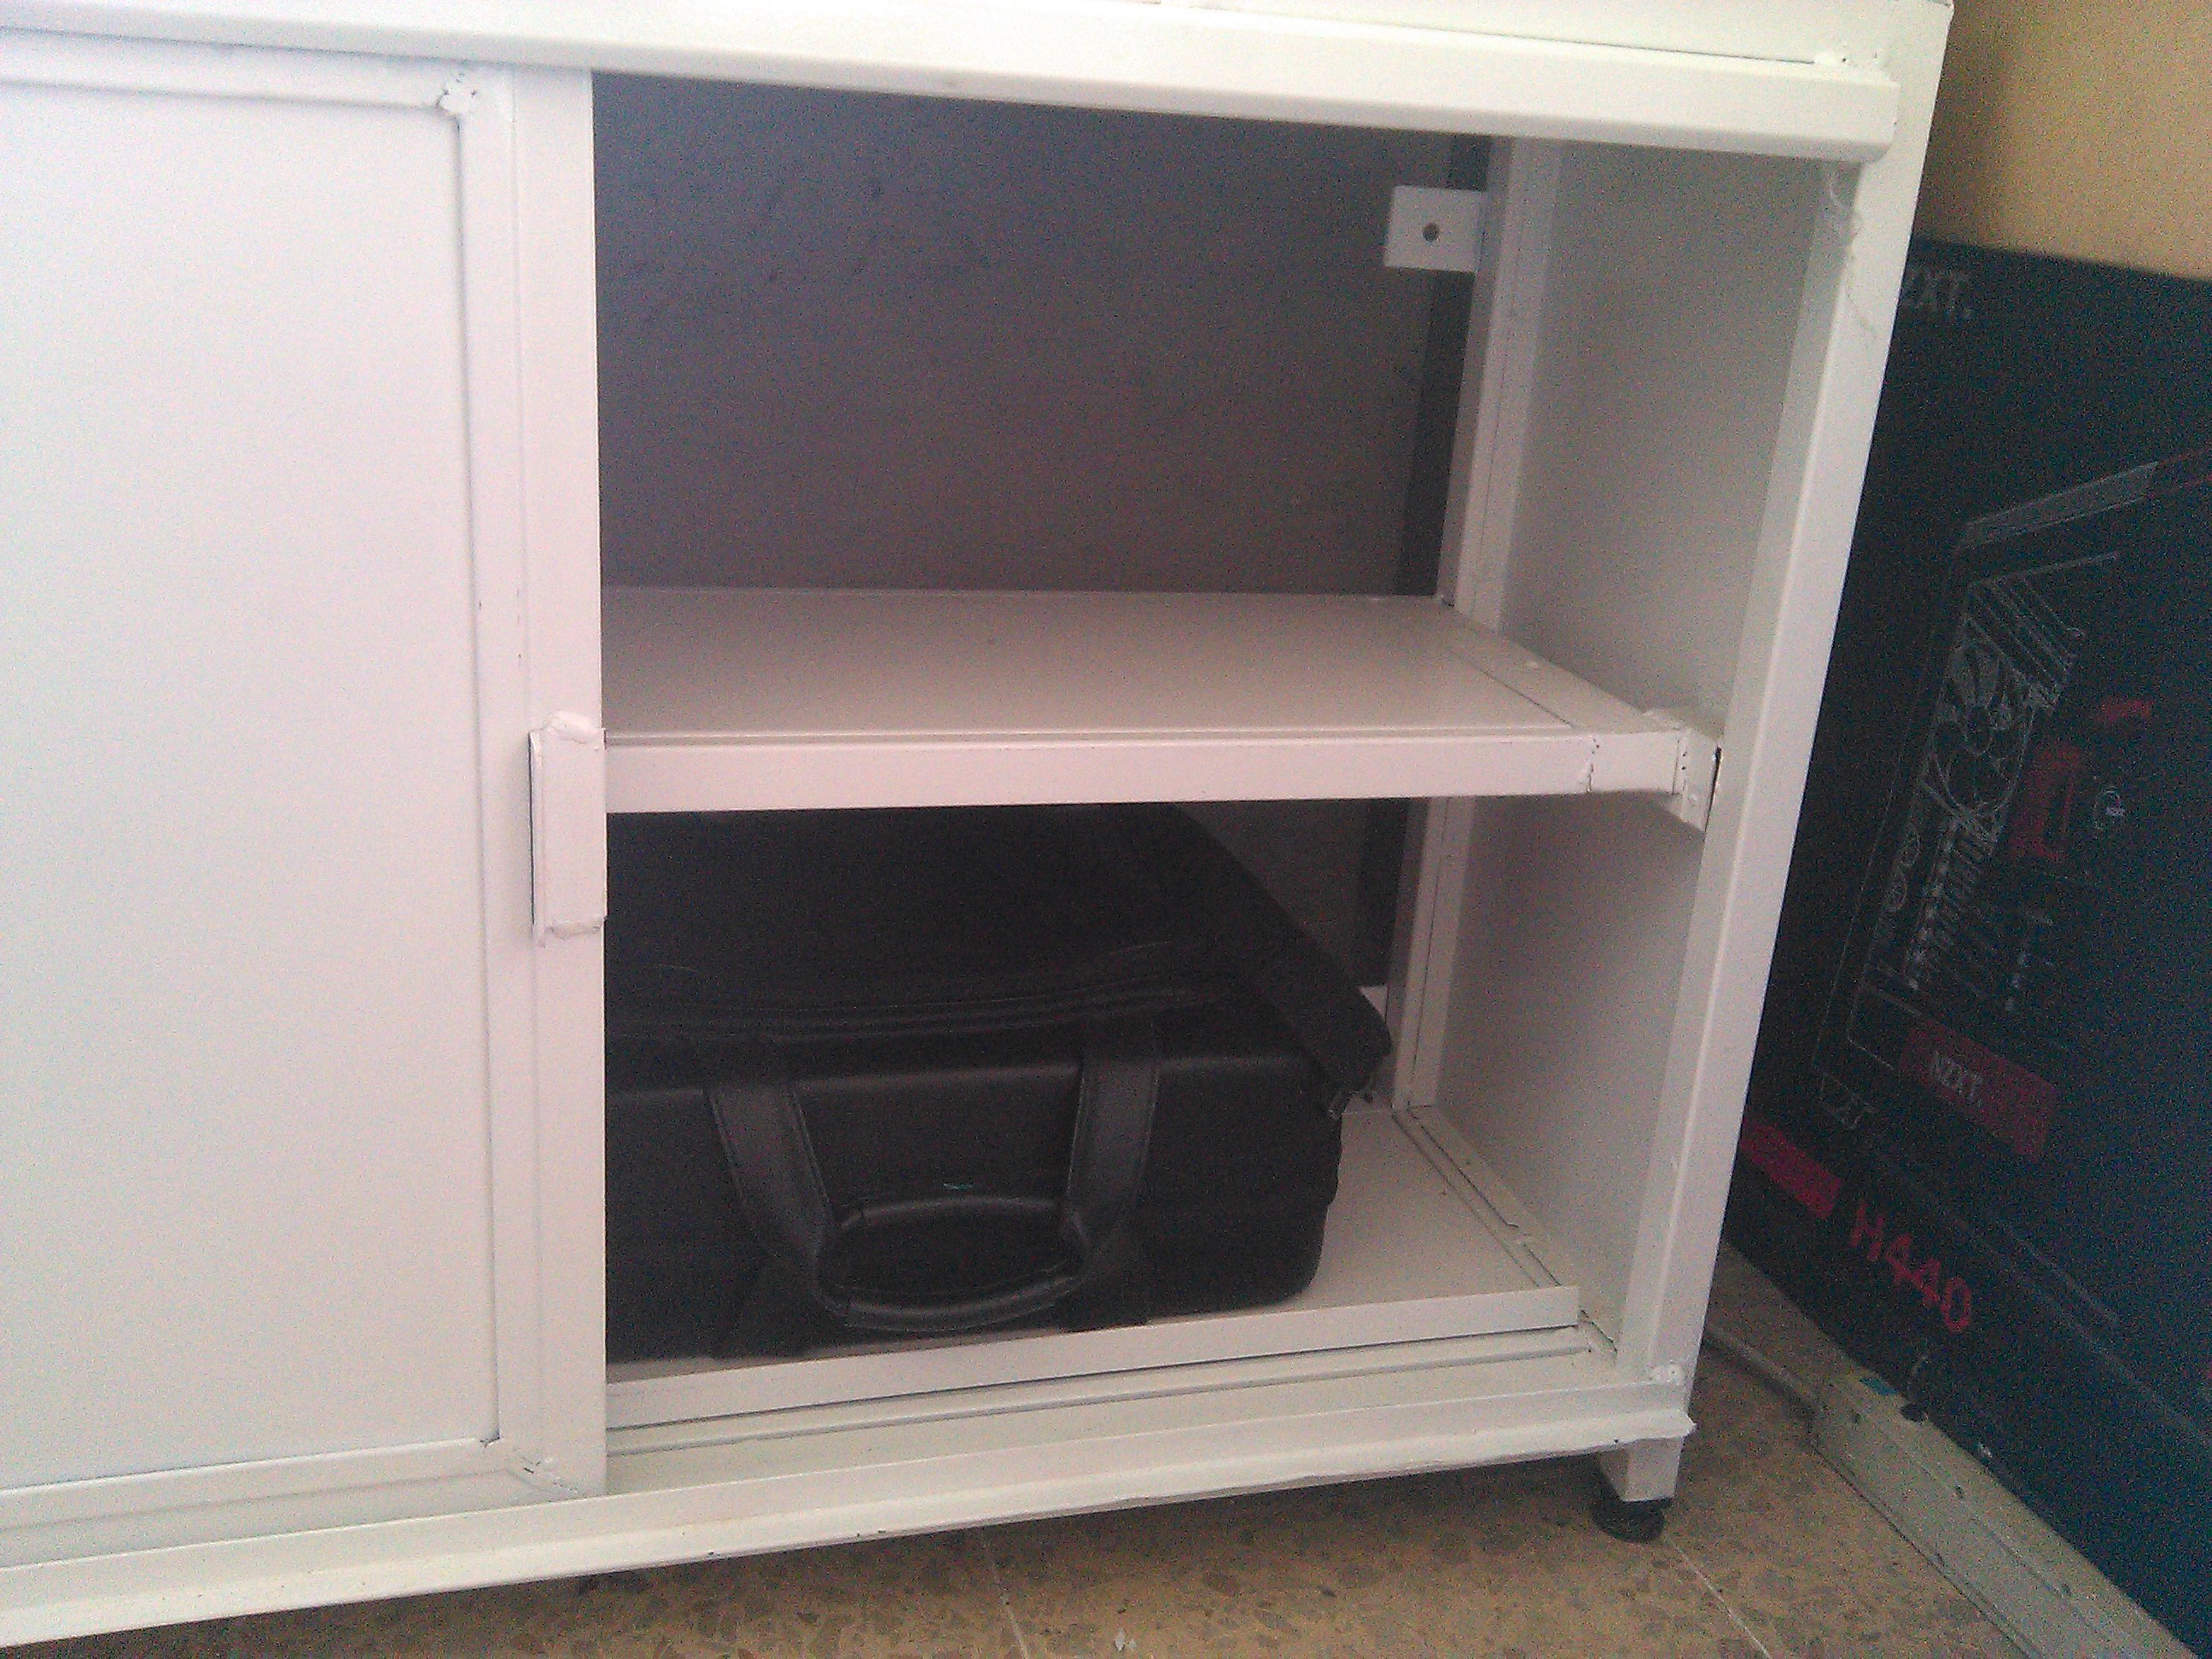
\includegraphics[width=0.2\textwidth]{images/anaquel-blanco-02}
      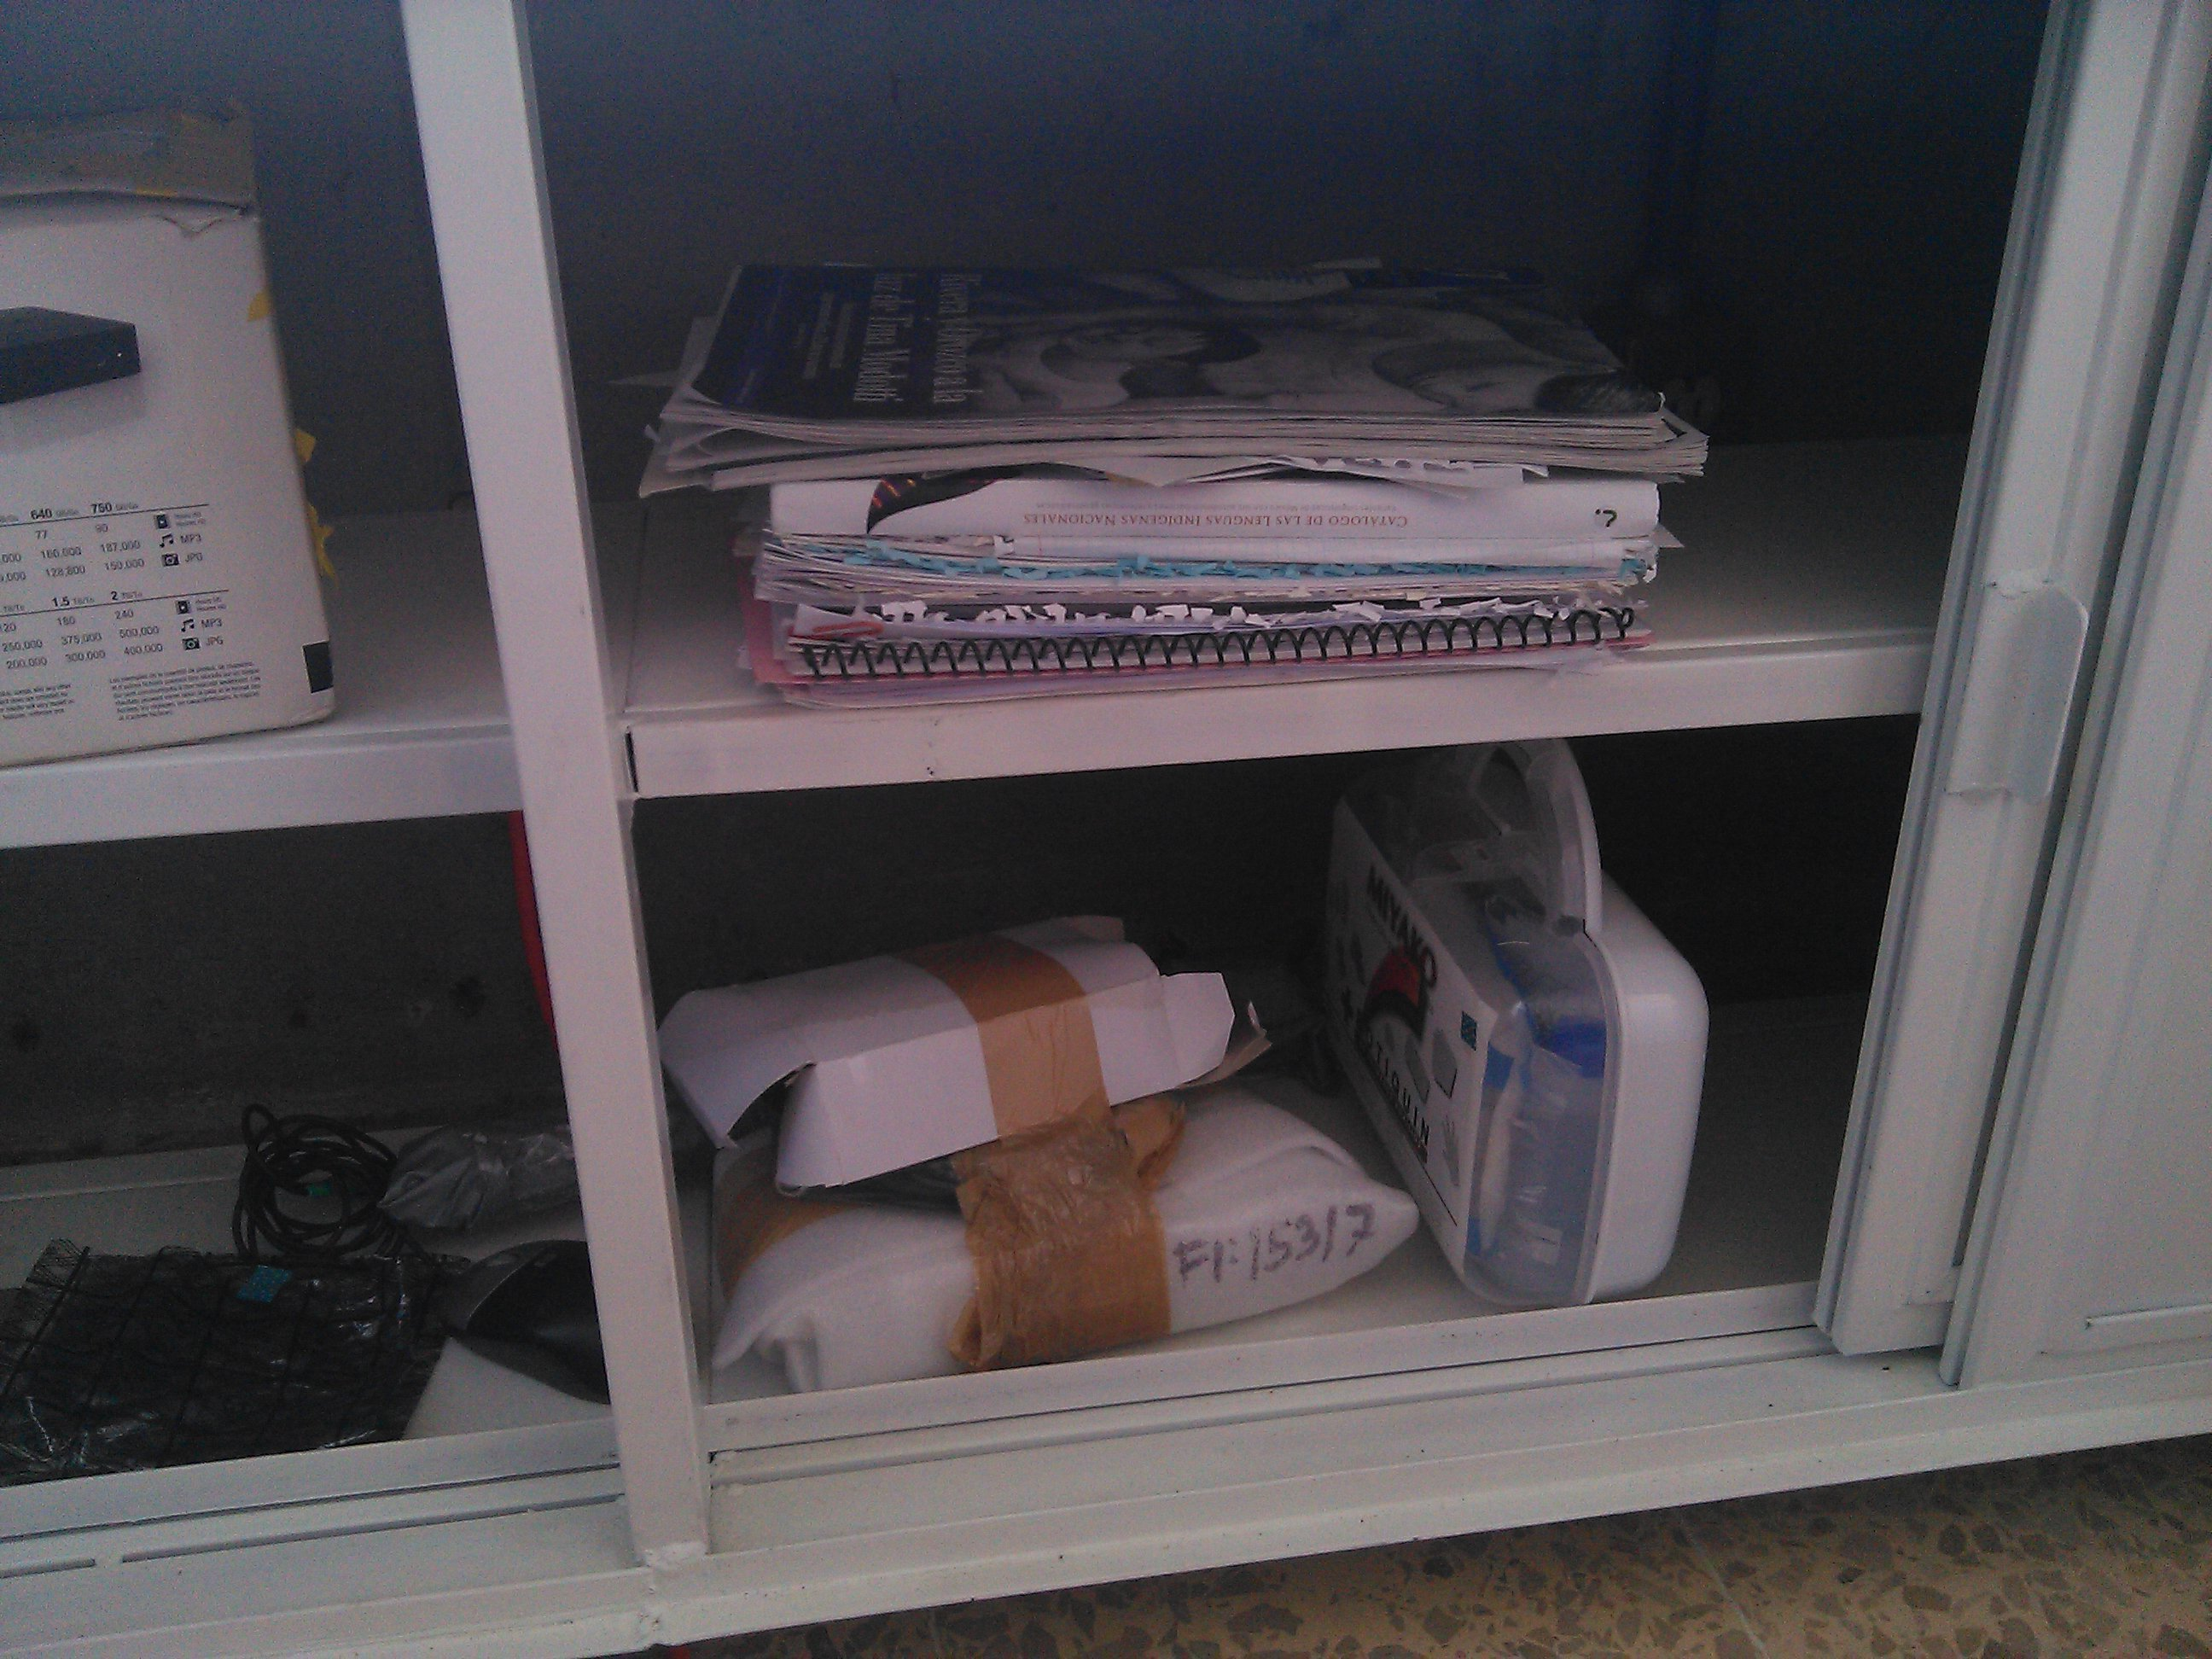
\includegraphics[width=0.2\textwidth]{images/anaquel-blanco-03}
      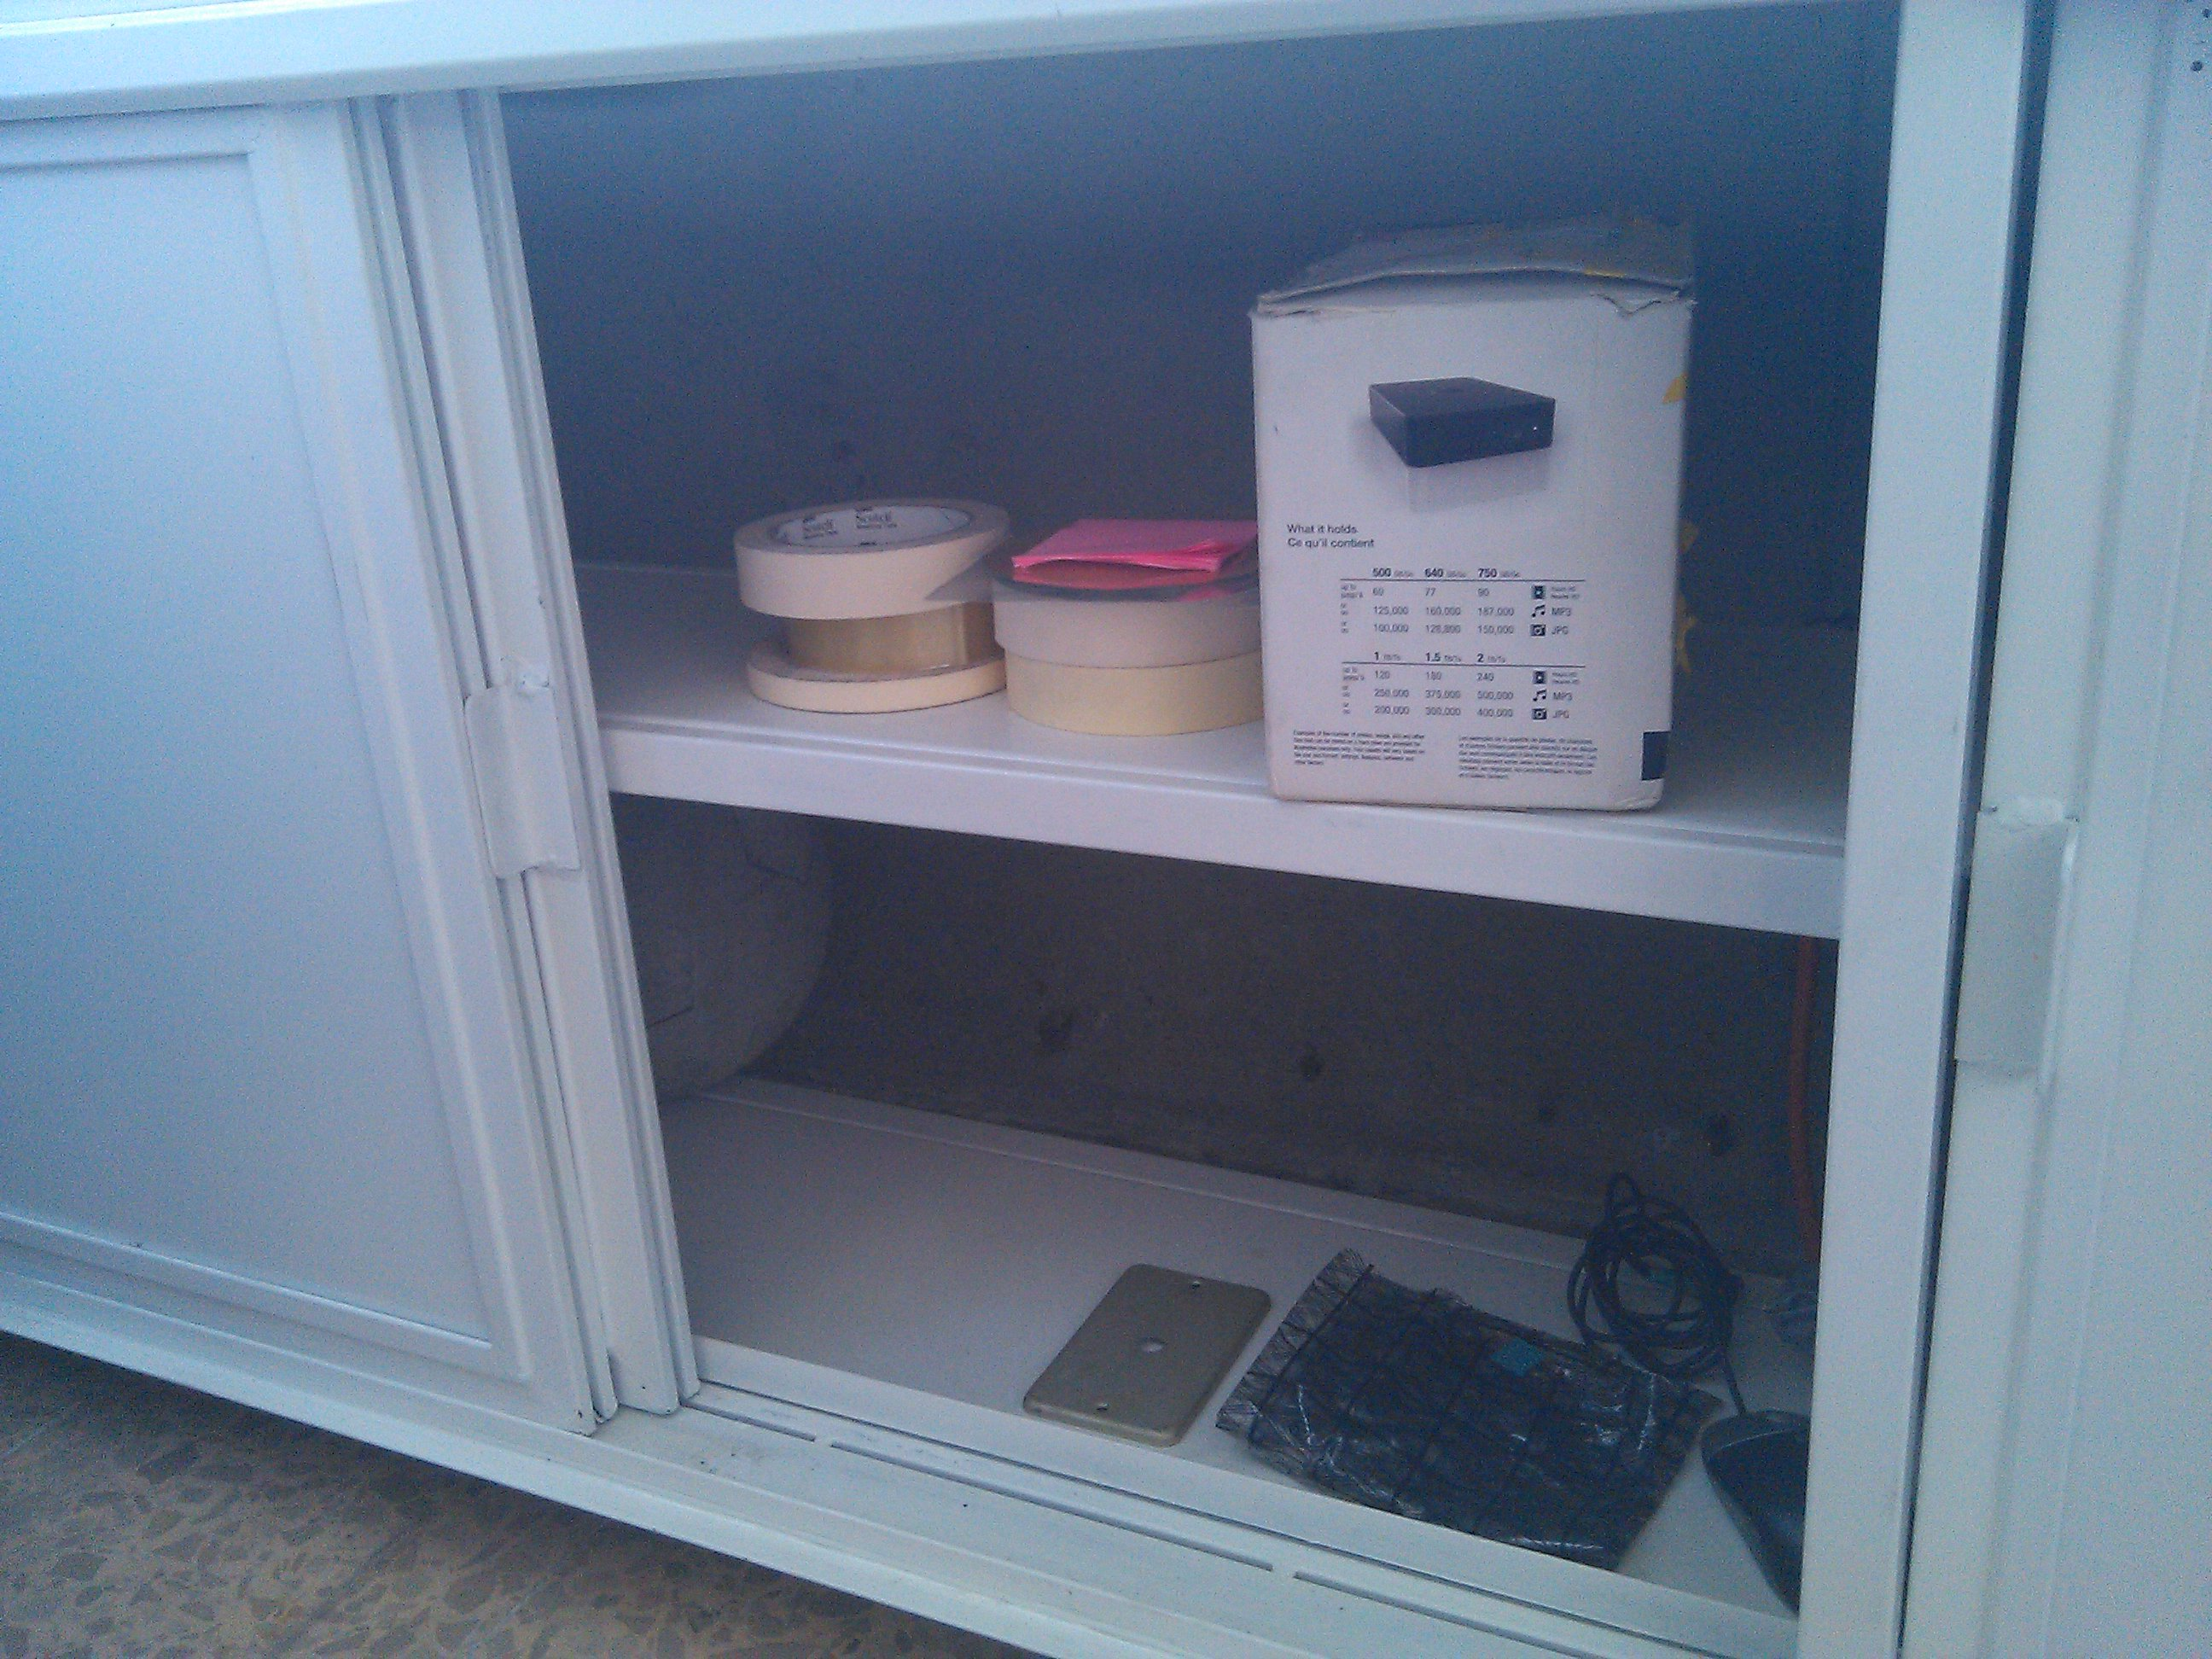
\includegraphics[width=0.2\textwidth]{images/anaquel-blanco-04} 
      \caption{Fotos del anaquel blanco}                       
   % \label{fig:bloque-tl-cero}                                  
    \end{figure}
  \subsubsection*{Anaquel gris}
    \begin{table}[H]
    \centering
    % \caption{My caption}
    % \label{my-label}
    \begin{tabular}{|c|l|}
    \hline
    Cantidad & Descripción                                        \\ \hline
    1        & Anaquel gris                                       \\ \hline
    1        & Multimetro Steren MUL400                           \\ \hline
    1        & Insecticida de 429 ml                              \\ \hline
    1        & Brocha para pintar 1 1/2”                          \\ \hline
    1        & Frasco con bicarbonato                             \\ \hline
    1        & Flexometro rojo                                    \\ \hline
    1        & Bote con tapa morada con componentes electrónicos  \\ \hline
    2        & Latas de calizador comex de 200 ml                 \\ \hline
    1        & Borrador para pintarron                            \\ \hline
    1        & Colección de libros (3 manuales técnicos, 7 tesis) \\ \hline
    1        & Bonche de hojas, carpetas, lijas, tabla de madera  \\ \hline
    1        & Cinta canela 2”                                    \\ \hline
    1        & Bote de pasta para soldar                          \\ \hline
    1        & Bote de `pintura vinil acrilica de 1l              \\ \hline
    2        & Juegos de cartas                                   \\ \hline
    1        & Paquete de 1000 grapas                             \\ \hline
    1        & Caja negra con componentes                         \\ \hline
    1        & Estuche naranja con componentes                    \\ \hline
    1        & Estuche transparente con componentes               \\ \hline
    1        & caja naranja con componentes                       \\ \hline
    1        & Recopilador verde                                  \\ \hline
    1        & Caja de herramientas gris grande                   \\ \hline
    1        & Bocina Logitech                                    \\ \hline
    1        & Juego de bocinas Logitech                          \\ \hline
    1        & Taza negra                                         \\ \hline
    1        & Bonche de carteles                                 \\ \hline
    1        & Swich Zchet                                        \\ \hline
    1        & Caja con productos comex                           \\ \hline
    2        & Latas de recubrimiento base comex de 800 ml        \\ \hline
    1        & Caja vacia de Router                               \\ \hline
    1        & Bonche de carteles, lona                           \\ \hline
    1        & Regulador                                          \\ \hline
    1        & Caja de herramientas gris chica                    \\ \hline
    \end{tabular}
    \end{table}
  \subsubsection*{Zona de trabajo}
    \begin{table}[H]
    \centering
    % \caption{My caption}
    % \label{my-label}
    \begin{tabular}{|c|l|}
    \hline
    Cantidad & Descripción                                                  \\ \hline
    1        & Cable HDMI                                                   \\ \hline
    1        & Cable ethernet 1 m                                           \\ \hline
    1        & Cable ethernet 12 m                                          \\ \hline
    1        & Extension Naranja                                            \\ \hline
    2        & Multicontactos (para las computadoras de la zona de trabajo) \\ \hline
    1        & Ventilador Honewell con control                              \\ \hline
    11       & Sillas negras ergonómicas                                    \\ \hline
    5        & Mesas de trabajo                                             \\ \hline
    1        & Bote de basura rectangular                                   \\ \hline
    1        & Banco de madera                                              \\ \hline
    1        & Refrigerador                                                 \\ \hline
    1        & Microondas                                                   \\ \hline
    1        & Cafetera                                                     \\ \hline
    1        & multicontacto (para refrigerador, cafetera y microondas)     \\ \hline
    1        & multicontacto (para panel azul)                              \\ \hline
    \end{tabular}
    \end{table}
  \subsubsection*{Equipos}
  \begin{table}[H]
\centering
%\caption{My caption}
%\label{my-label}
\begin{tabular}{|c|l|}
\hline
Cantidad & Descripción                                                                                                                                                                                                         \\ \hline
2        & Monitor Dell 20” y cables de alimentación*                                                                                                                                                                          \\ \hline
2        & \begin{tabular}[c]{@{}l@{}}CPU’s Slim Dell Inspiron 560s \\ \\ y cable de alimentación*\end{tabular}                                                                                                                \\ \hline
2        & Cables VGA                                                                                                                                                                                                          \\ \hline
2        & Teclados Dell                                                                                                                                                                                                       \\ \hline
2        & Mouse Dell                                                                                                                                                                                                          \\ \hline
1        & \begin{tabular}[c]{@{}l@{}}Equipo Dell “Zombie” con S.O. Fedora 15,\\ usuario Roberto, Pentium, 64 bits, 4GB de memoria\end{tabular}                                                                                \\ \hline
1        & \begin{tabular}[c]{@{}l@{}}Equipo HP Compaq “Rompope” con S.O. Debian 8, \\ AMD ATHLONX2, 64 bits, (corriendo) está conectado \\ a la red “Metztli”\end{tabular}                                                    \\ \hline
1        & \begin{tabular}[c]{@{}l@{}}Equoi con case negro NZXT (computadora armada) \\ “LIDSOL” con S.O. Debian 8, está conectado a la red \\ “Juan Carreon”, además tiene un repetidor LINKSYS\\  modelo EA2700\end{tabular} \\ \hline
1        & Monitor HP L1710                                                                                                                                                                                                    \\ \hline
1        & Teclado HP                                                                                                                                                                                                          \\ \hline
1        & Caja transparente con varios cables                                                                                                                                                                                 \\ \hline
\end{tabular}
\end{table}

\newpage
  \subsection{Inventario a Mayo 2018}
  \subsubsection{Hadware y otros.}




% Please add the following required packages to your document preamble:
% \usepackage{multirow}
% \usepackage[table,xcdraw]{xcolor}
% If you use beamer only pass "xcolor=table" option, i.e. \documentclass[xcolor=table]{beamer}
%\begin{table}[]
%\centering
%\caption{My caption}
%\label{my-label}

\begin{longtable}{|p{.15\textwidth}|p{.3\textwidth}|p{.1\textwidth}|p{.1\textwidth}|p{.15\textwidth}|p{.12\textwidth}|}
\hline
                           &                                                &                                                                              &                             &                                                                                 &                               \\
\multirow{-2}{*}{Cantidad} & \multirow{-2}{*}{Artículo}                     & \multirow{-2}{*}{\begin{tabular}[c]{@{}l@{}}Inventario \\ UNAM\end{tabular}} & \multirow{-2}{*}{Estado}    & \multirow{-2}{*}{Comentarios}                                                   & \multirow{-2}{*}{Procedencia} \\ \hline
\multicolumn{6}{|l|}{\cellcolor[HTML]{EFEFEF}{\color[HTML]{343434} Monitores y Pantallas}}                                                                                                                                                                                                                 \\ \hline
6                          & Monitores HP L1710                             & -                                                                            & Funcional                   & Sin cables                                                                      & LIDSOL                        \\ \hline
1                          & Monitor HP 2511t                               & -                                                                            & Funcional                   & Sin cables                                                                      & LIDSOL                        \\ \hline
                           &                                                &                                                                              &                             &                                                                                 &                               \\
\multirow{-2}{*}{1}        & \multirow{-2}{*}{Pantalla LED 32" LG 32lf550b} & \multirow{-2}{*}{15249}                                                      & \multirow{-2}{*}{Funcional} & \multirow{-2}{*}{\begin{tabular}[c]{@{}l@{}}Con control \\ remoto\end{tabular}} & \multirow{-2}{*}{LIDSOL}      \\ \hline
1                          & Monitor DELL in2010nb                          & 02318454                                                                     & Funcional                   & Sin cables                                                                      & LIDSOL                        \\ \hline
1                          & Monitores DELL in2010nb                        & 02318453                                                                     & Funcional                   & Sin cables                                                                      & LIDSOL                        \\ \hline
\multicolumn{6}{|l|}{\cellcolor[HTML]{EFEFEF}{\color[HTML]{343434} Computadoras y Laptops}}                                                                                                                                                     \\ \hline
1                          & DELL Inspiron 560S                    & 2318452                                                                      & Funcional                   & -                             & LIDSOL                        \\ \hline
1                          & DELL Inspiron 560S                    & 2318451                                                                      & Funcional                   & -                             & LIDSOL                        \\ \hline
                           &                                       &                                                                              &                             &                               &                               \\
\multirow{-2}{*}{1}        & \multirow{-2}{*}{DELL Dimension 5150} & \multirow{-2}{*}{2226268}                                                    & \multirow{-2}{*}{Funcional} & \multirow{-2}{*}{-}           & \multirow{-2}{*}{LIDSOL}      \\ \hline
1                          & Laptop ACER vx15                      & 2495850                                                                      & Funcional                   & -                             & LIDSOL                        \\ \hline
\multicolumn{6}{|l|}{\cellcolor[HTML]{EFEFEF}{\color[HTML]{343434} Perifericos}}                                                                                                                                                     \\ \hline
2                          & Teclados DELL sk-8185         & -                                                                            & Funcional                & -                             & LIDSOL                        \\ \hline
2                          & Mouse DELL ms111p             & -                                                                            & Funcional                & -                             & LIDSOL                        \\ \hline
1                          & Bocinas LOGITEC z313          & -                                                                            & Funcional                & Un Sub buffer y dos bocinas   & LIDSOL                        \\ \hline
1                          & Audifonos SENNHEISER          & -                                                                            & Funcional                & -                             & LIDSOL                        \\ \hline
1                          & Audifonos BEATS powerbeats    & -                                                                            & Funcional                & Estuche y extensor            & LIDSOL                        \\ \hline
1                          & No break ISB                  & -                                                                            & Funcional                & -                             & LIDSOL                        \\ \hline
1                          & Impresora Laser Jet HP p1102w & -                                                                            & Funcional                & Con cable y sin tinta         & LIDSOL                        \\ \hline
\multicolumn{6}{|l|}{\cellcolor[HTML]{EFEFEF}{\color[HTML]{343434} Redes}}                                                                                                                                                                                                \\ \hline
1                          & Switch ZONET zfs3016                    & -                                                                            & Desconocido              & -                                                        & LIDSOL                        \\ \hline
2                          & Tarjetas inalambricas TPLINK tl-wn781nd & -                                                                            & Funcional                & Instaladas                                               & LIDSOL                        \\ \hline
2                          & Tarjetas inalambricas TPLINK tl-wn751nd & -                                                                            & Funcional                & No instaladas                                            & LIDSOL                        \\ \hline
1                          & Transmisor fm                           & 15317                                                                        & Funcional                & Eliminador, cable de corriente, cable de antena y antena & LIDSOL                        \\ \hline
1                          & Router ENGENIUS esr600                  & -                                                                            & Funcional                & -                                                        & LIDSOL                        \\ \hline
1                          & Router LINXYS ea2700                    & -                                                                            & Funcional                & -                                                        & LIDSOL                        \\ \hline
1                          & Cable UTP                               & -                                                                            & Funcional                & 5.5 metros                                               & LIDSOL                        \\ \hline
\multicolumn{6}{|l|}{\cellcolor[HTML]{EFEFEF}{\color[HTML]{343434} Cables}}                                                                                                                                                                      \\ \hline
1                          & Rollo de cable plano de 26 hilos & -                                                                            & -                        & -                                      & LIDSOL                        \\ \hline
1                          & Caja de cables varios            & -                                                                            & -                        & Caja transparente sobre el mueble gris & LIDSOL                        \\ \hline
3                          & Multicontactos                   & -                                                                            & -                        & -                                      & LIDSOL                        \\ \hline
1                          & Extensión de uso rudo            & -                                                                            & -                        & -                                      & LIDSOL                        \\ \hline
1                          & Extensión regular                & -                                                                            & -                        & -                                      & LIDSOL                        \\ \hline
                           &                                                &                                                                              &                             &                                                                                 &                               \\
\multirow{-2}{*}{Cantidad} & \multirow{-2}{*}{Artículo}                     & \multirow{-2}{*}{\begin{tabular}[c]{@{}l@{}}Inventario \\ UNAM\end{tabular}} & \multirow{-2}{*}{Estado}    & \multirow{-2}{*}{Comentarios}                                                   & \multirow{-2}{*}{Procedencia} \\ \hline
\multicolumn{6}{|l|}{\cellcolor[HTML]{EFEFEF}{\color[HTML]{343434} Varios}}                                                                                                                                                                                                                                \\ \hline
1                          & Insecticida H24                                                                       & -                                                                            & -                        & -                                           & LIDSOL                        \\ \hline
1                          & Bote de pintura blanca                                                                & -                                                                            & -                        & 1 litro                                     & LIDSOL                        \\ \hline
3                          & Botes de catalizador Sketch                                                           & -                                                                            & -                        & 200 ml cada uno                             & LIDSOL                        \\ \hline
3                          & Botes de recubrimiento base Sketch                                                    & -                                                                            & -                        & 800 ml cada uno                             & LIDSOL                        \\ \hline
1                          & Taza medidora Sketch                                                                  & -                                                                            & -                        & -                                           & LIDSOL                        \\ \hline
1                          & Aromatizante                                                                          & -                                                                            & -                        & Bote casi vacio                             & LIDSOL                        \\ \hline
1                          & Caja de herramienta pequeña negro/gris, broches amarillo                              & -                                                                            & -                        & -                                           & LIDSOL                        \\ \hline
2                          & Desarmador plano                                                                      & -                                                                            & -                        & -                                           & LIDSOL                        \\ \hline
1                          & Desarmador phillips                                                                   & -                                                                            & -                        & -                                           & LIDSOL                        \\ \hline
1                          & Lima                                                                                  & -                                                                            & -                        & -                                           & LIDSOL                        \\ \hline
2                          & Desarmador con cabeza intercambiable                                                  & -                                                                            & -                        & -                                           & LIDSOL                        \\ \hline
1                          & Pinzas plateadas                                                                      & -                                                                            & -                        & -                                           & LIDSOL                        \\ \hline
1                          & Caja de herramienta Rimax grande gris, broches amarillos                              & -                                                                            & -                        & -                                           & LIDSOL                        \\ \hline
1                          & Caja transparente pequeña con cables, tornillos y cosillas varias                     & -                                                                            & -                        & -                                           & LIDSOL                        \\ \hline
1                          & Caja transparente durazno pequeña con compuertas lógicas, display 7 segmentos         & -                                                                            & -                        & -                                           & LIDSOL                        \\ \hline
1                          & Caja naranja, tapa transparente con capacitores, push button, motores, potenciometros & -                                                                            & -                        & -                                           & LIDSOL                        \\ \hline
1                          & Caja negra con componentes electricos (resistencias)                                  & -                                                                            & -                        & -                                           & LIDSOL                        \\ \hline
1                          & Caja de gises                                                                         & -                                                                            & -                        & -                                           & LIDSOL                        \\ \hline
1                          & Carpeta Tamaño oficio verde                                                           & -                                                                            & -                        & -                                           & LIDSOL                        \\ \hline
1                          & Estuche transparente con hojas blancas                                                & -                                                                            & -                        & -                                           & LIDSOL                        \\ \hline
5                          & Tazas café                                                                            & -                                                                            & -                        & -                                           & LIDSOL                        \\ \hline
1                          & Jabon liquido verde                                                                   & -                                                                            & -                        & -                                           & LIDSOL                        \\ \hline
1                          & Zacate verde                                                                          & -                                                                            & -                        & -                                           & LIDSOL                        \\ \hline
1                          & Bolsa de café                                                                         & -                                                                            & -                        & -                                           & LIDSOL                        \\ \hline
1                          & Botiquin de primeros auxilios                                                         & -                                                                            & Medio funcional          & Falta alcohol                               & LIDSOL                        \\ \hline
1                          & Extintor                                                                              & -                                                                            & Descono- cido              & Ultima inspección fue el 31 de Mayo de 2017 & LIDSOL                        \\ \hline

\multicolumn{6}{|l|}{\cellcolor[HTML]{EFEFEF}{\color[HTML]{343434} Mobiliario}}                                                                                                                                                                                                \\ \hline
11                         & Sillas con ruedas          & -                                                                            & Funcional                & -                                                                          & LIDSOL                        \\ \hline
1                          & Banco                      & -                                                                            & Funcional                & -                                                                          & LIDSOL                        \\ \hline
\newpage
\hline
                           &                            &                                                                              &                          &                                                                            &                               \\
\multirow{-2}{*}{Cantidad} & \multirow{-2}{*}{Artículo} & \multirow{-2}{*}{\begin{tabular}[c]{@{}l@{}}Inventario \\ UNAM\end{tabular}} & \multirow{-2}{*}{Estado} & \multirow{-2}{*}{Comentarios}                                              & \multirow{-2}{*}{Procedencia} \\ \hline

5                          & Mesas de trabajo           & -                                                                            & Funcional                & Color café claro donde se trabaja                                          & LIDSOL                        \\ \hline

1                          & Pizzarrón blanco           & -                                                                            & Funcional                & -                                                                          & LIDSOL                        \\ \hline
1                          & Refrigerador               & -                                                                            & Funcional                & -                                                                          & LIDSOL                        \\ \hline
1                          & Horno de microondas        & -                                                                            & Funcional                & -                                                                          & LIDSOL                        \\ \hline
1                          & Cafetera                   & -                                                                            & Funcional                & -                                                                          & LIDSOL                        \\ \hline
1                          & Estante gris               & -                                                                            & Funcional                & -                                                                          & LIDSOL                        \\ \hline
1                          & Aire acondicionado         & -                                                                            & Funcional                & -                                                                          & LIDSOL                        \\ \hline
1                          & Mueble grande de madera    & -                                                                            & Funcional                & Hecho a la medida del laboratorio                                          & LIDSOL                        \\ \hline
\multicolumn{6}{|l|}{\cellcolor[HTML]{EFEFEF}{\color[HTML]{343434} Externo}}                                                                                                                                                                                                                                                                      \\ \hline
1                          & AlienWare d07u                            & 2471577                                                                      & Funcional                & Eliminador y cable HDMI                                                    & Dr. Rodrigo Montufar Chaveznava (Colaboración PAPIME PE216116)                    \\ \hline
1                          & Mouse y teclado inalambricos DELL 580addv & -                                                                            & Funcional                & Con receptor inalambrico parte de AlienWare                                & Dr. Montufar                                                                      \\ \hline
1                          & Control XBOX 360                          & -                                                                            & Funcional                & Parte de AlienWare                                                         & Dr. Montufar                                                                      \\ \hline
1                          & DELL xps 8910                             & 2488874                                                                      & Funcional                & -                                                                          & Dr. Montufar                                                                      \\ \hline
1                          & Oculus Rift                               & 2491027                                                                      & Funcional                & Incluye receptor y control inalambrico.                                    & Dr. Montufar                                                                      \\ \hline
1                          & Control XBOX ONE                          & -                                                                            & Funcional                & Con receptor inalabrico y cable de extension                               & Dr. Montufar                                                                      \\ \hline
2                          & Touch Controllers de Oculus Rift          & -                                                                            & Funcional                & -                                                                          & Dr. Montufar                                                                      \\ \hline
2                          & Receptor inalambrico para Oculus Rift     & -                                                                            & Funcional                & -                                                                          & Dr. Montufar                                                                      \\ \hline
1                          & Accesorio para RockBand                   & -                                                                            & Funcional                & -                                                                          & Dr. Montufar                                                                      \\ \hline
1                          & Audifonos para Oculus Rift                & -                                                                            & Funcional                & -                                                                          & Dr. Montufar                                                                      \\ \hline
1                          & LEAP Motion                               & -                                                                            & Funcional                & Incluye dos cables USB 3.0, un extensor de USB 3.0 y base para oculus Rift & Dr. Montufar                                                                      \\ \hline
\newpage
\hline
                           &                                           &                                                                              &                          &                                                                            &                                                                                   \\
\multirow{-2}{*}{Cantidad} & \multirow{-2}{*}{Artículo}                & \multirow{-2}{*}{\begin{tabular}[c]{@{}l@{}}Inventario \\ UNAM\end{tabular}} & \multirow{-2}{*}{Estado} & \multirow{-2}{*}{Comentarios}                                              & \multirow{-2}{*}{Procedencia}                                                     \\ \hline
1                          & Visores Marvel CARDBOARD                  & -                                                                            & Funcional                & -                                                                          & Dr. Montufar                                                                      \\ \hline

1                          & Visor SAMSUNG Gear VR                     & -                                                                            & Funcional                & Incluye adaptador de USB-C a microUSB                                      & Dr. Montufar                                                                      \\ \hline


1                          & Celular SAMSUNG Galaxy S5                 & -                                                                            & Funcional                & Incluye cable y cargador                                                   & Dr. Montufar                                                                      \\ \hline
1                          & Fpga Altera de2i-150                      & -                                                                            & Funcional                & Incluye eliminador                                                         & Emilio Cabrera                                                                    \\ \hline
1                          & Rack azul                                 & -                                                                            & Funcional                & -                                                                 & M.C. Alejandro Velázquez Mena, Jefe del Departamento de Ingeniería en Computación \\ \hline
2                          & DELL se2417hg                             & -                                                                            & Funcional                & Cable de alimentacion y cable VGA                                          & En rack azul y se desconoce propietario                                            \\ \hline

\end{longtable}
%\end{table}

  \subsubsection{Libros, revistas y documentación.}
  
\begin{longtable}{|p{.15\textwidth}|p{.73\textwidth}|p{.12\textwidth}|}
\hline
Cantidad & Descripción                                                                                                                                               & Procedencia \\ \hline
1        & Marco normativo de la defensoria de los derechos universitarios                                                                                        & LIDSOL      \\ \hline
1        & Libro IA-32 intel architecture optimization reference manual                                                                                           & LIDSOL      \\ \hline
1        & Libro IA-32 intel software developer's manual. Volumen 2B                                                                                              & LIDSOL      \\ \hline
1        & Memoria de la feria de proyectos 2013                                                                                                                  & LIDSOL      \\ \hline
1        & Ingeniería. Investigación y tecnología Vol XIV Num 2 jul-sept 2013                                                                                     & LIDSOL      \\ \hline
1        & Tesis Deteccion de espectro para radio cognitiva en frecuencias de television mediante radio definido por software.  Autor: Ing Monica Alcaraz Vadillo & LIDSOL      \\ \hline
1        & Tesis Membranas fotolimunicentes electrohiladas para detccción UVA. Autor: Jorge Alberto Gutierrez Mena                                                & LIDSOL      \\ \hline
1        & Tesis Procesos de señal de television digital en banda KU utilizado en Mexico y latinoamerica a inicios del siglo XXI. Autor: Adolfo Medina Barrera.   & LIDSOL      \\ \hline
1        & Tesis Sistema automatizado de iluminación de una casa mediante comandos de voz. Autor: Francisco Navarrete Tolento                                     & LIDSOL      \\ \hline
1        & Practica 2: Introducción a GNU radio. Lab de television digital terrestre basado en software definido por radio. Autor Miguel Angel Alvarado Zaragoza  & LIDSOL      \\ \hline
1        & Borrador de tesis Procesos de señal de television digital en banda KU utilizado en Mexico y latinoamerica a inicios del siglo XXI                      & LIDSOL      \\ \hline
1        & Documento con herramientas y prácticas de ciberseguridad                                                                                               & LIDSOL      \\ \hline
1        & Tesis replicación simétrica, un cazo avanzado de las bases de datos Oracle, un ejemplo de su aplicación. Autor: Tapia Corona Rodrigo                   & LIDSOL      \\ \hline
\newpage
\hline
Cantidad & Descripción                                                                                                                                               & Procedencia \\ \hline
1        & Tesis Sistema de administración escolar de la facultad de ingeniería. Autor: Jose Luis Estrada Salas                                                   & LIDSOL      \\ \hline
1        & Tesis desarrollo de framework para interacción con llaves asimétricas en aplicaciones Web. Autor: Guillermo Romero Gallegos                            & LIDSOL      \\ \hline

\end{longtable}


    
  \section{Miembros}
  \begin{itemize}
    \item Juan José Carreón Granados
    
    Profesor fundador de LIDSOL.
    
    \item Gunnar Wolf 
    
    Es el nuevo responsable académico, dirige el \textbf{Proyecto PAPIME PE102718 - Desarrollo de materiales didácticos para los mecanismos de privacidad y anonimato en redes}. Más información de este proyecto \href{https://www.priv-anon.unam.mx/}{aquí}, \href{https://github.com/LIDSOL/papime-pe102718-mecanismos-de-privacidad-y-anonimato}{repositorio}. Tiene llaves del Laboratorio.
    
    \item Andrés Hérnandez
    
    Ingeniero en computación, es colaborador académico.
    
    \item Aguilar Enriquez Paul Sebastian
    
    Estudiante de Ingeniería en computación, tiene intereses en las áreas de inteligencia artificial, procesamiento de lenguaje natural, recuperación de información, lenguas indigenas y seguridad digital. Comenzó con la reestructuración del laboratorio en Octubre de 2016, al mismo tiempo inició el reclutamiento de nuevos miembros.  Hizo su servicio social y trajó consigo la colaboración del  \textbf{Proyecto PAPIME PE216116 - Ambientes virtuales y herramientas digitales para neurociencia}. Invitó al profesor Gunnar Wolf a colaborar de manera formal y académica en el laboratorio y como fruto de esto se inicio el \textbf{Proyecto PAPIME PE102718 - Desarrollo de materiales didácticos para los mecanismos de privacidad y anonimato en redes} en colaboración con LIDSOL. Inicio el contacto con el \href{https://issuu.com/nigromantefi}{\textbf{Nigromante  (Revista DCSyH FI  UNAM)}} para las colaboraciones mensuales. Dio una conferencia sobre \textbf{la historia del software libre y los hackers} en la (\textbf{Feria de Agrupaciones de la FI}), y escribió un artículo sobre el mismo tema para el \href{https://issuu.com/nigromantefi}{\textbf{Nigromante  (Revista DCSyH FI  UNAM)}}. Impartió un taller sobre \href{https://github.com/LIDSOL/nightlynight}{\textbf{Cómo contribuir a Nightly (Firefox)}} en la (\textbf{Feria de Agrupaciones de la FI}) como parte de un proyecto que se realiza en el laboratorio en conjunto con la comunidad \textbf{Mozilla México}, de donde es miembro. Tiene llaves del Laboratorio.
    
    \item Barriga Martínez Diego Alberto
    
    Estudiante de Ingeniería en computación, becario del \textbf{Proyecto PAPIME PE102718 - Desarrollo de materiales didácticos para los mecanismos de privacidad y anonimato en redes}. Hablo sobre \textbf{Derechos digitales} en una conferencia en conjunto con Gunnar en la (\textbf{Feria de Agrupaciones de la FI}), y escribió un artículo sobre \textbf{La neutralidad de la red} para el \href{https://issuu.com/nigromantefi}{\textbf{Nigromante  (Revista DCSyH FI  UNAM)}}. Impartió un taller sobre \href{https://github.com/umoqnier/personal-page}{\textbf{Github pages}} en el laboratorio. Tiene llaves del Laboratorio.
    
    \item Cabrera Lopez Oscar Emilio 
    
    Estudiante de Ingeniería en computación, es \textbf{Sysadmin} de los servidores del laboratorio, es becario del \textbf{Proyecto PAPIME PE216116 - Ambientes virtuales y herramientas digitales para neurociencia}, dicho proyecto es coordinado por el profesor Rodrigo Montufar Chaveznava y se hace en colaboración con LIDSOL, \href{https://github.com/LIDSOL/portia}{(ver repositorio)}. Realizo el guión de los \href{https://www.youtube.com/channel/UCwHFqMqxUcCAJSdek3e4zOw}{vídeos} que se publicaron en torno al  \textbf{Proyecto PAPIME -PE104415}. Impartió un \href{https://lidsol.org/talleres/0002_css_basico.html}{taller de css} en el laboratorio y un taller de administración de una impresora 3D en la (\textbf{Feria de Agrupaciones de la FI}). Tiene llaves del Laboratorio.
    
    \item Flores Gaspar Juan Antonio
    
    Estudiante de Ingeniería en computación, becario del \textbf{Proyecto PAPIME PE102718 - Desarrollo de materiales didácticos para los mecanismos de privacidad y anonimato en redes}, interesado en seguridad informatica. 
    

    \item Navarro Yesica 
    
    Estudiante de Inegiería eléctrica electrónica, entusiasta del software y las tecnologías libres, coordina colaboraciones de LIDSOL con el \href{https://issuu.com/nigromantefi}{\textbf{Nigromante  (Revista DCSyH FI  UNAM)}} mensualmente, \href{https://github.com/LIDSOL/material-didactico/tree/master/nigromante}{ver repositorio}. Participó activamente en la logística del último evento (\textbf{Feria de Agrupaciones de la FI}),  impartiendo en el mismo un \href{https://github.com/yesn7/taller-kicad/}{\textbf{Taller de KiCad}}. Realizo la edición de los \href{https://www.youtube.com/channel/UCwHFqMqxUcCAJSdek3e4zOw}{vídeos} que se publicaron en torno al  \textbf{Proyecto PAPIME -PE104415}. Tiene llaves del Laboratorio.
    
    \item Oropeza Vilchis Luis Alberto
    
    Estudiante de Ingeniería en computación, es becario del \textbf{Proyecto PAPIME PE216116 - Ambientes virtuales y herramientas digitales para neurociencia}, dicho proyecto es coordinado por el profesor Rodrigo Montufar Chaveznava y se hace en colaboración con LIDSOL, \href{https://github.com/LIDSOL/portia}{(ver repositorio)}. Participó activamente en la (\textbf{Feria de Agrupaciones de la FI}), ayudando en el installfest y reclutando a nuevos miembros en los stands. Tiene llaves del Laboratorio.
    
    \item Perez Hernandez Nohemi
    
    Estudiante de Ingeniería geofísica, está interesada en desarrollo 3D. Participó en la (\textbf{Feria de Agrupaciones de la FI}), ayudando en la logística del evento. Colabora activamente en el \href{https://github.com/LIDSOL/OpenSCAD-free-models}{\textbf{Proyecto \textit{Modelos libres de OpensCAD}}} coordinado por Pablo Vivar.
    
    \item Rios Morales Alexis Manuel
    
    Estudiante de Ingeniería en computación. Participó en la (\textbf{Feria de Agrupaciones de la FI}), apoyando como voluntario a los encargados del installfest y  los stands.
     
    \item Ruano Muñoz Marco Antonio
    
    Estudiante de Ingeniería en computación, becario del \textbf{Proyecto PAPIME PE102718 - Desarrollo de materiales didácticos para los mecanismos de privacidad y anonimato en redes}. Publicó en la \textbf{Revista .Seguridad} el artículo \href{https://revista.seguridad.unam.mx/numero30/la-red-tor-como-elemento-de-privacidad-en-nuestras-vidas}{La red Tor como elemento de privacidad en nuestras vidas}. Tiene llaves del Laboratorio.
    
    \item Torres Rosales Luz Olimpia
    
    Estudiante de Ingeniería eléctrica electrónica. Participó en la (\textbf{Feria de Agrupaciones de la FI}), apoyando como voluntario a los a los talleristas. Fungió como voz en \href{https://www.youtube.com/channel/UCwHFqMqxUcCAJSdek3e4zOw}{vídeos} que se publicaron en torno al  \textbf{Proyecto PAPIME -PE104415}.
    
    \item Vivar Colina Pablo
    
    Estudiante de Ingeniería eléctrica electrónica. Está interesado en el desarrollo 3D, y tiene un proyecto propio en el laboratorio (\href{https://github.com/LIDSOL/OpenSCAD-free-models}{\textbf{Proyecto \textit{Modelos libres de OpensCAD}}}), por lo mismo intenta reclutar personas al final de los distintios \href{https://github.com/LIDSOL/OpenSCAD-curso}{talleres de OpensCAD} que ha impartido en el laboratorio. Tiene llaves del Laboratorio.
  \end{itemize}
  
  \section{Necesidades}
  \begin{itemize}
    \item Un garrafón con agua, así como de un mueble para colocarlo o de una bomba para extraer agua del garrafón. Este servicio ya lo tienen todos los laboratorios aledaños.
    \item Diez marcadores para pizarrón blanco, pues siempre se hacen anotaciones constantemente en el pizarrón. 
    \item Cinco extensiones y cinco multicontactos, pues los actuales ya no satisfacen a todas las personas que visitan el laboratorio con regularidad.
    \item Cinco llaveros, para colocar las llaves de los anaqueles, del baño, etc.
    \item Un plumero, pues aunque si pasan a hacer la limpieza, no la hacen a profundidad y los miembros podrían ayudar en este aspecto si se contara con uno.
    \item Cuatro computadoras, pues las actuales ya no satisfacen a todas las personas que visitan el laboratorio con regularidad.
    \item Un aire acondicionado, o bien 
    \item Un servidor, pues los actuales están muy viejos y no son hadware dedicado.
    \item Cinco canaletas para cableado de red, pues los cables atraviesan el laboratorio sin protección y de una forma un poco insegura.
    \item Un proyector de tiro corto así como de un soporte para proyector.
    \item \textit{Necesidades de los miembros de LIDSOL.}

    ALgunos miembros del laboratorio quieren una beca pues están en condiciones para recibirla, otros quisieran liberar su servivio social.

    \item \textit{Necesidades solucionadas.}

    La puerta de acceso al laboratorio ya fue reparada. El wifi funciona bien. Las sillas que hay en el laboratorio ya son suficientes. Ya fue retirado el nido de avispas ubicado en la parte exterior de la ventana.

  \end{itemize}
  \section{Actividades}
  
  
  
  
   
%%%%%%%%%%%%%%%%%%%%%%%%%%%%%%%%%%%%%%%%%%%%%%%%%%%%%%%%%%%%%%%%%%%%%%%%%%%%%%%%%%%%%%%%%
  


%%%%%%%%%%%%%%%%%%%%%%%%%%%%%%%%%%%%%%%%%%%%%%%%%%%%%%%%%%%%%%%%%%%%%%%%%%%%%%%%%%%%%%%%%

\end{document}
